\documentclass[journal,twocolumn]{IEEEtran}
\usepackage{graphicx}
\graphicspath{{figures/}}
\DeclareGraphicsExtensions{.pdf,.jpeg,.png}
\usepackage{amsmath, amssymb}
\usepackage{float}
\usepackage{url}
\usepackage[hidelinks]{hyperref}
\hypersetup{
	linktoc=all
}
\usepackage[T1]{fontenc}
\usepackage[utf8]{inputenc}
\usepackage{authblk}
\usepackage{physics}
\usepackage[normalem]{ulem}
\useunder{\uline}{\ul}{}
\hyphenation{op-tical net-works semi-conduc-tor}
\usepackage[sorting=none, backend=bibtex]{biblatex}
\nocite{*}
\addbibresource{references}

\begin{document}

\title{Shallow-learning methods for pedestrian classification and detection in images}

\author[1]{Master’s degree in Computer Engineering for Robotics and Smart Industry\\Machine Learning and Artificial Intelligence course, a.a. 2021/2022\\ Lorenzo Busellato}%
\affil[1]{VR472249, lorenzo.busellato\_02@studenti.univr.it}
\onecolumn

\maketitle
\begin{abstract} Pedestrian detection is a key task in the computer vision field, given its obvious applications in surveillance systems, autonomous driving and robotics. 
This work presents a pipeline for shallow-learning based pedestrian detection. The Histogram of Oriented Gradients (HOG)
method for feature extraction is described and applied to the Daimler Mono Pedestrian Classification Benchmark Data Set. Three classification
techniques, Support Vector Machines (SVMs), K-Nearest Neighbors (KNN) and Naive Bayes, are described and benchmarked
with different sets of hyperparameters. The benchmarks are then compared against each other to determine the best performing
method in terms of accuracy in classification. Finally the best performing classifier is showcased by using it in a full pipeline for pedestrian detection applied to a video sequence.
\end{abstract}
  \tableofcontents
  \listoffigures
  \listoftables  
  \clearpage
  \twocolumn

\IEEEpeerreviewmaketitle

\section{Introduction}
\IEEEPARstart{T}{he} task of pedestrian detection, i.e. the task of localizing pedestrians within an image, is one of the most tackled
instances of the broader class of object detection problems.
This is due to its natural applications in autonomous driving,
surveillance and robotics. For instance, in the US alone about
5000 of the 35000 annual car accident fatalities involve
pedestrians \cite{1}, therefore the need for automated methods for
pedestrian detection is apparent.

The task of pedestrian detection presents a series of complexities regarding the high variability in scale and size of the
person within the image, occlusions with the rest of the scene,
susceptibility to lighting conditions and the real time detection
requirement.

The main models that are used for pedestrian detection are
hand-crafted models and deep learning models. Hand-crafted
models are based on classification of hand-crafted features. Deep learning models on the other hand typically use
convolutional neural networks for the extraction of features,
therefore producing high-level semantic representations of
objects.
In this work the first class of models will be analyzed
and implemented. Specifically, the Histogram of Oriented
Gradients (HOG) method will be used to extract features from
images, because it is known\cite{2} that it is the best performing non-deep learning based feature extractor for human detection. The classification of images will then be implemented
using non-deep learning methods, namely Support Vector
Machines (SVMs), K-Nearest Neighbors (KNN) and Naive Bayes. Finally the best performing classifier will be used
to implement a pedestrian detector.

The details of the implementation can be found on the project's GitHub page\cite{4}.

The main objectives of this work are described in section
\ref{sec:obj}. The data set and methodology employed are described in
sections \ref{sec:data} and \ref{sec:meth}. The experimental evaluation is presented
in section \ref{sec:exp}. The conclusions are summarized in section \ref{sec:conc}.

\section{Objectives}
\label{sec:obj}
The main objective of this work is the implementation of
a pedestrian detection pipeline, which is made up
of three main components: a feature extractor, a classifier and a
detector.

Regarding the classifiers, the objective is to obtain an in-depth comparison between the performance of some well-known shallow learning techniques with respect to the problem of pedestrian detection, as well as the relation between hyperparameters and classifier performance.

Finally, the best performing classifier will be used to implement a detector, therefore completing the pedestrian detection pipeline. The pipeline will then be applied to a video sequence in order to showcase its performance.

\section{Dataset}
\label{sec:data}

The data set used in this work is the Daimler Mono Pedestrian Classification Benchmark Data Set\cite{3}. The data set consists of four separate subsets: the base set and three additional sets. The base set is divided into five subsets, three for training (named "1", "2" and "3") and two for testing (named "T1" and "T2"). All five sets contain 4800 18$\times$36 grayscale images containing pedestrians and 5000 18$\times$36 grayscale images not containing pedestrians. The three additional sets each contain 1200 640$\times$280 grayscale images for the purpose of extracting additional negative samples for the hard-negative mining procedure.

\begin{figure}[h]
\begin{minipage}{0.45\columnwidth}
\centering
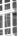
\includegraphics[keepaspectratio,width=0.4\textwidth]{1}
\end{minipage}
\begin{minipage}{0.45\columnwidth}
\centering
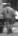
\includegraphics[keepaspectratio,width=0.4\textwidth]{2}
\end{minipage}
\caption[Example images from the dataset]{Example figures from the training data set. On the left a non-pedestrian sample, on the right a pedestrian sample.}
\end{figure}

In this work, data sets 1, 2 and 3 will be grouped together in a singular data set for the training of the models, as will data sets T1 and T2 for the testing.

\section{Methodology}
\label{sec:meth}

\subsection{Histogram of Oriented Gradients}

Given an input image $I$, for each pixel $(x,y)\in I$ the gradients $G_x$ and $G_y$ are computed. This is typically done via a convolution operation:

\begin{equation*}
G_x=\omega_x* I\;\;\;\;\;G_y=\omega_y* I
\end{equation*}

where $\omega_x$ and $\omega_y$ are the kernels associated to the convolution operation. The most common kernels used in the context of pedestrian detection are:

\begin{equation*}
\omega_x=\begin{bmatrix}
-1 & 0 & 1
\end{bmatrix}\;\;\;\;\;\omega_y=\omega_x^T
\end{equation*}

They are the most commonly used because experimentally it is observed\cite{2} that they produce the least amount of detected false positives per moving window (FFPW) compared to other kernels.

After the convolution operation, two gradient matrices are obtained, $G_x$ and $G_y$. For each pixel $(x,y)\in I$ then the magnitude $\mu$ and angle $\theta$ are computed:

\begin{equation*}
\mu(i,j)=\sqrt{G_x(i,j)^2+G_y(i,j)^2}
\end{equation*}

\begin{equation*}
\theta(i,j)=\abs{\tan^{-1}\left(\frac{G_y(i,j)}{G_x(i,j)}\right)}
\end{equation*}

In practice the angle is computed with $atan2$, therefore it is in the range $(\pi,\pi]$.

The resulting gradient magnitude and gradient angle matrices are then divided into $8\times 8$ patches, for each of which a 9-point histogram of oriented gradients is computed. A
histogram is a series of bins labeled with angle values. The
number of bins is determined by the angle step between
the bins, for instance with an angle step of 20 degrees the
histogram will have $180^\circ/20^\circ = 9$ bins.

For each pixel in the patch, the corresponding gradient angle
determines two bins on the histogram that the pixel votes for.
The two bins selected are those which represent the two closest
angles to the given gradient angle value. The value added to
the selected bins is proportional to the distance of the gradient
angle to the bin angle, the gradient magnitude and the step
between the bins:
\begin{equation*}
v_{closest}=\frac{(binAngle-\theta)\mu}{angleStep}
\end{equation*}
\begin{equation*}
v_{2nd-closest}=\frac{(\theta-binAngle)\mu}{angleStep}
\end{equation*}

Repeating the process for each 8 × 8 patch, a 16$\times$8 matrix
of histograms is constructed.
To reduce the variability in gradient intensities due to lighting conditions and foreground-background contrast, a block
normalization procedure is introduced. The 16$\times$8 histogram
matrix is scanned with a 2$\times$2 window producing 15$\times$7 blocks,
for each of which a normalized histogram vector is computed
by concatenating the four histograms contained in the block
and normalizing the resulting vector.
Finally, the feature descriptor for the image is constructed
by concatenating the normalized histogram vectors. From
each 8$\times$8 patch a 1$\times$9 vector is collected, which is then
concatenated with another three 1$\times$9 vectors composing a
1$\times$36 vector, which is finally concatenated with another
fourteen 1$\times$36 vectors, resulting in a 1$\times$3780 feature vector.

\begin{figure}[h]
\centering
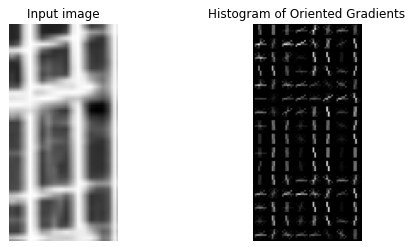
\includegraphics[keepaspectratio,width=0.9\columnwidth]{3}
\caption[HOG representation of a non-pedestrian sample]{Histogram of Oriented Gradients representation of a non-pedestrian sample.}
\label{fig:3}
\end{figure}
\begin{figure}[h]
\centering
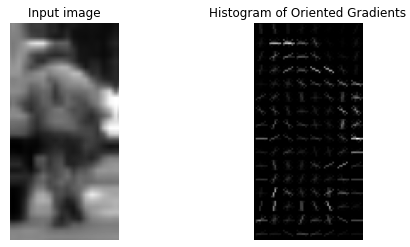
\includegraphics[keepaspectratio,width=0.9\columnwidth]{4}
\caption[HOG representation of a pedestrian sample]{Histogram of Oriented Gradients representation of a pedestrian sample.}
\label{fig:4}
\end{figure}

A representation of the resulting feature vector can be seen in figures \ref{fig:3} and \ref{fig:4}. The representation is obtained by plotting the 9$\times$1 normalized histograms in each 8$\times$8 cell. The dominant direction of the histogram is able to capture contours, especially straight lines such as the frame of the window in figure \ref{fig:3} or the legs of the pedestrian in figure \ref{fig:4}. The gradient magnitudes also carry information on the lighting of the scene, with greater magnitudes corresponding to lighter areas.

\subsection{Naive Bayes}

Naive Bayes is a class of supervised learning methods based on the "naive" assumption that each pair of features is conditionally independent given the value of the class variable.

Given the class variable $y$ and the dependent feature vector $x=(x_1,\dots,x_n)$, Bayes' theorem states that:
\begin{equation}
P(y\mid x_1,\dots, x_n)=\frac{P(y)P(x_1,\dots,x_n\mid y)}{P(x_1,\dots,x_n)}
\end{equation}

Under the conditional independence assumption that for all $i$:
\begin{equation*}
P(x_i\mid y,x_1,\dots,x_{i-1},x_{i+1},\dots, x_n)=P(x_i\mid y)
\end{equation*}

the theorem reduces to:
\begin{equation*}
P(y\mid x_1,\dots, x_n)=\frac{P(y)\prod\limits_{i=1}^nP(x_i\mid y)}{P(x_1,\dots,x_n)}
\end{equation*}

Since $P(x_1,\dots,x_n)$ is constant given the input, and acts only as a scaling factor:

\begin{equation*}
P(y\mid x_1,\dots, x_n)\propto P(y)\prod\limits_{i=1}^nP(x_i\mid y)
\end{equation*}

Therefore the following classification rule can be derived:

\begin{equation*}
\hat y = \underset{y}{argmax}P(y)\prod\limits_{i=1}^nP(x_i\mid y)
\end{equation*}

$P(y)$ and $P(x_i\mid y)$ are derived via maximum a posteriori estimation.

The different naive Bayes classifier differ only with respect to the chosen shape of the distribution of $P(x_i\mid y)$. In this work only Gaussian Naive Bayes will be considered. The model assumes that the likelihood distribution of the features is Gaussian:

\begin{equation*}
P(x_i\mid y)=\frac{1}{\sqrt{2\pi\sigma_y^2}}exp\left(-\frac{(x_i-\mu_y)^2}{2\sigma_y^2}\right)
\end{equation*}

where the mean $\mu_y$ and variance $\sigma_y$ are obtained using maximum likelihood estimation.

\subsection{K-Nearest Neighbors}

K-Nearest Neighbors (KNN) is a non-parametric supervised learning method used for classification. It is based on the assumption that feature vectors belonging to the same class are close
together in the feature space. Given an unlabeled sample,
the distance from it to every sample in the training set is
computed using some metric, typically euclidean. The label
of the sample is then given by the mode of the K samples
with the smallest distance from the unlabeled sample. The
algorithm is as follows:
\begin{itemize}
\item Initialize K as the desired number of neighbors.
\item For each sample in the training data set, compute the
distance between the unknown sample and the current
sample and add it to a list.
\item Sort the list of distances and pick the first K entries.
\item The label for the unknown sample is the mode of the
labels of the K entries.
\end{itemize}
Regarding
the choice of K, a common heuristic is to pick $K=\sqrt{N}$, where N is the number of training samples. A more robust approach is to repeat the training of the model
with varying K values, among which a "best" one is to be
selected with respect to the minimization of some error metric, typically accuracy. In this work the second approach will be employed, showing that choosing the square root of the number of samples is not always the best option in terms of accuracy.

Another choice to be made is the adopted distance metric. In
this work the Minkowski metric will be used. The Minkowski
metric of order $p$, where $p$ is an integer, between two points $X=(x_1,\dots,x_n)\in\mathbb{R}^n$ , $Y=(y_1,\dots,y_n) \in\mathbb{R}^n$ is defined
as:

\begin{equation*}
D(X,Y)=\left(\sum\limits_{i=1}^n\abs{x_i-y_i}^p\right)^{\frac{1}{p}}
\end{equation*}

For $p=1$ the metric reduces to the so-called Cityblock metric, which is the sum of the absolute differences of the cartesian coordinates of the points. For $p=2$ the metric reduces to the Euclidean distance. In this work the model will be employed with $p=1,2,3$, showing the differences in classifier performance in the three cases.

\subsection{Support Vector Machines}

Support Vector Machines (SVMs) are a class of supervised learning algorithms whose main idea is to find an optimal hyperplane in an $n$-dimensional space, with $n$ number of features, that maximizes the distance, called margin, between the classes of data points. Such an hyperplane constitutes the decision boundary used by a classifier to classify data points, on the basis of which "side" of the hyperplane they fall in. The position and orientation of the hyperplane are influenced by the data points closer to it, which are called support vectors.




\subsection{Hard-negative mining}

\subsection{Pedestrian detection}

To detect pedestrian in a given input image, a sliding window approach is used. Firstly, a Gaussian Pyramid is extracted
from the image. That is to say the image is progressively
downsampled, obtaining a set of lower resolution versions of the input image at every scale.

\begin{figure}[H]
\centering
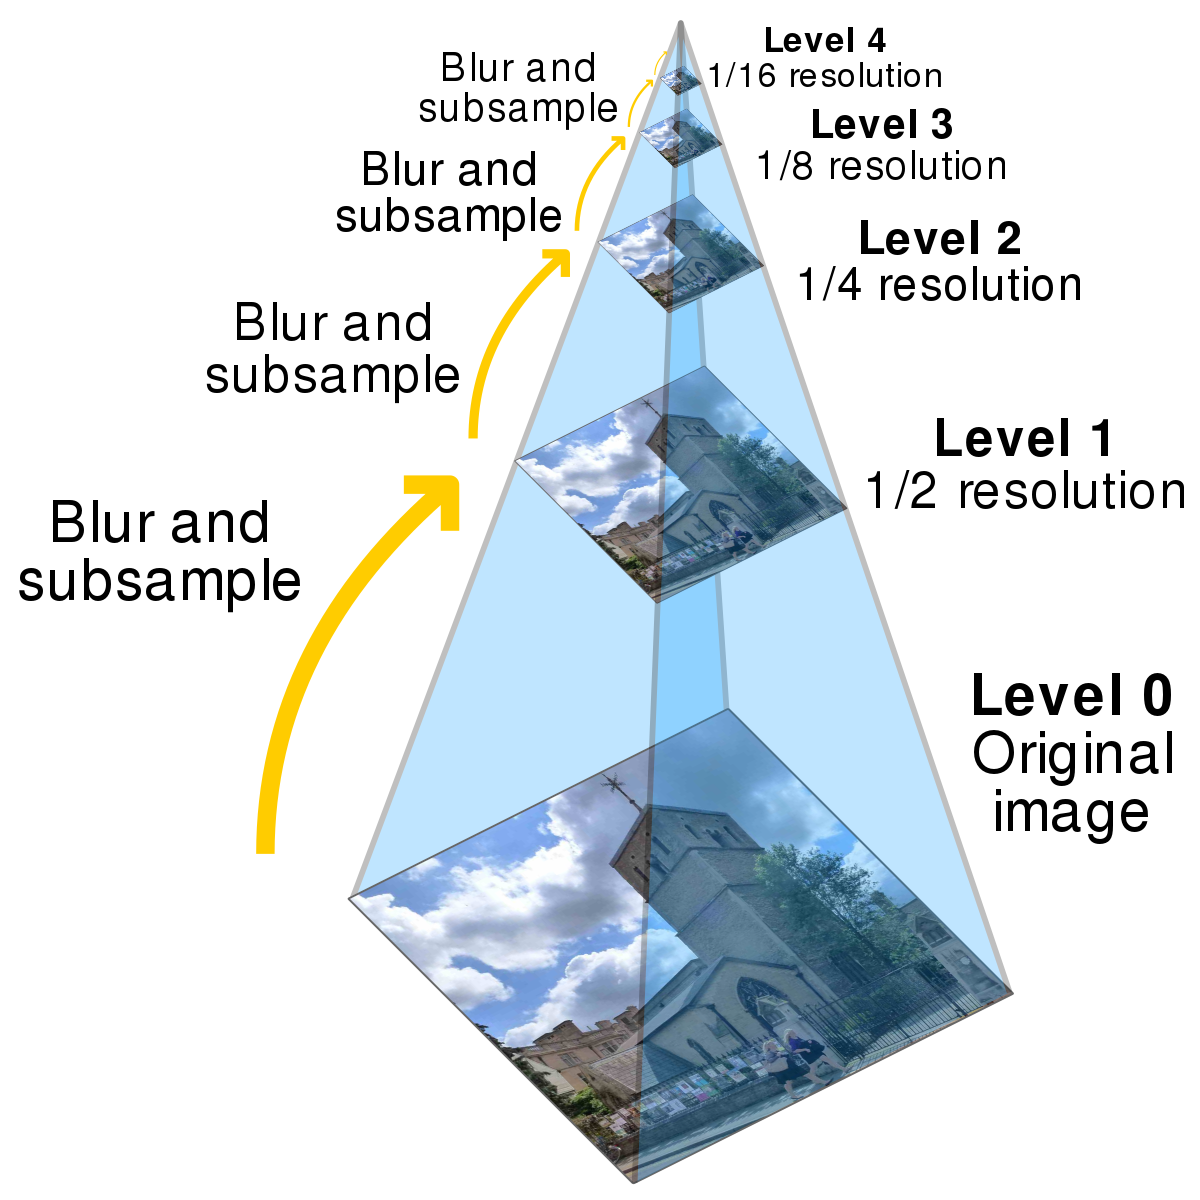
\includegraphics[keepaspectratio,width=0.35\textwidth]{5}
\caption{Gaussian pyramid}
\end{figure}

Then, a sliding window is passed over each image in the
pyramid, and a HOG feature vector is computed for each step
of the sliding.
Finally, the feature vector is classified by one of the
previously described classifiers. If the classifier identifies the
window as a pedestrian, the coordinates of its top left corner
as well as the confidence score and its properly scaled width
and height, define the bounding box around the pedestrian.
This approach, while effective in locating pedestrians within
an image, produces multiple proposals for the bounding box.
This is because windows that contain only a portion of a
pedestrian still can produce feature vectors similar to those produced by windows that fully capture a pedestrian.

\subsection{Non-maximum suppression}

Non-maximum suppression (NMS) is a technique for the
filtering of predictions made by an object detector. An object
detector typically produces a list B of proposed bounding
boxes along with the confidence score S assigned to each of
them. The algorithm is as follows:
\begin{itemize}
\item Select from B the proposal with the highest confidence
score, remove it from B, and add it to an initially empty
list D.
\item Compare the proposal with all other proposals in D by
computing the Intersection Over Union (IOU):
\begin{equation*}
IOU=\frac{\text{Intersection Area}}{\text{Total Area}}
\end{equation*}
\item Remove from B all the proposals with an IOU greater
than some threshold.
\item Repeat steps 1-3 until B is empty.
\end{itemize}

The list D then contains only the bounding boxes that have the highest confidence score and that intersect the least with other bounding boxes already in D.

\section{Experiments and results}
\label{sec:exp}

\subsection{Adopted metrics}

To evaluate the performance of the various classifiers, the following metrics were used:

\begin{itemize}
\item Accuracy:
\begin{equation*}
Accuracy=\frac{TP+TN}{TP+FP+FN+TN}
\end{equation*}
Accuracy is a raw evaluation of the number of correct guesses with respect to the total number of samples. It is well suited for binary classification problems such as pedestrian classification, but it can be misleading for the detection phase since in an image the pedestrian labels are typically sparse.
\item Precision:
\begin{align*}
Precision_P &= \frac{TP}{TP+FP}\\
Precision_N &= \frac{TN}{TN+FN}
\end{align*}
Precision is the proportion of predicted positives (or negatives) that actually are positive (or negative) samples. It is an important metric for pedestrian detection because the pipeline needs to limit as much as possible wrong detections, which could be problematic for applications like autonomous driving.
\item Recall:
\begin{align*}
Recall_P &= \frac{TP}{TP+FN}\\
Recall_N &= \frac{TN}{TN+FP}
\end{align*}
Recall is the proportion of actual positives correctly classified. It is an important metric for pedestrian detection because the pipeline needs to correctly classify as many pedestrians as possible in a given image (hopefully all of them).
\item $F_1$ score:
\begin{equation*}
F_1=2\frac{Precision_P\times Recall_P}{Precision_P + Recall_P}
\end{equation*}
$F_1$ offers a trade-off between precision and recall. It is a perfectly suited metric for pedestrian detection because the pipeline needs to both maximize the detection rate, but also be sure that the detections actually are pedestrians, or in other words the higher the $F_1$ score, the better. For these reasons only the $F_1$ score related to the pedestrian label is calculated.
\end{itemize}

where TP is the number of true positives, TN the number of true negatives, FP the number of false positives and FN the number of false negatives detected by the classifier.

\subsection{Performed experiments}

\subsection{Results}

\begin{table}[H]
\caption{Measured metrics for Naive Bayes}
\begin{tabular}{cccccc}
\hline\\ [-1.5ex]
{Accuracy} & Precision NP & Precision P & Recall NP & Recall P & $F_1$ score \\ \hline\\ [-1.5ex]
87.52          & 0.854        & 0.901       & 0.912     & 0.837  &0.867  \\ \hline\\ [-1.5ex]
\end{tabular}
\end{table}

\section{Conclusions}
\label{sec:conc}

\printbibliography


\end{document}